\documentclass[12pt]{article}

\usepackage[spanish]{babel}
\usepackage[utf8]{inputenc}
\usepackage{graphicx}
\usepackage{geometry}
\usepackage{xcolor}
\usepackage{fancyhdr}
\usepackage{lastpage}
\usepackage{pdfpages}
\usepackage{listings}
\usepackage{schemata}

\geometry{top=25mm,left=15mm,right=15mm,a4paper}

\pagestyle{fancy}
\fancyhf{}
\lhead{Redes de Computadoras}
\cfoot{Página \thepage\ de \pageref{LastPage}}

\graphicspath{./}

\begin{document}
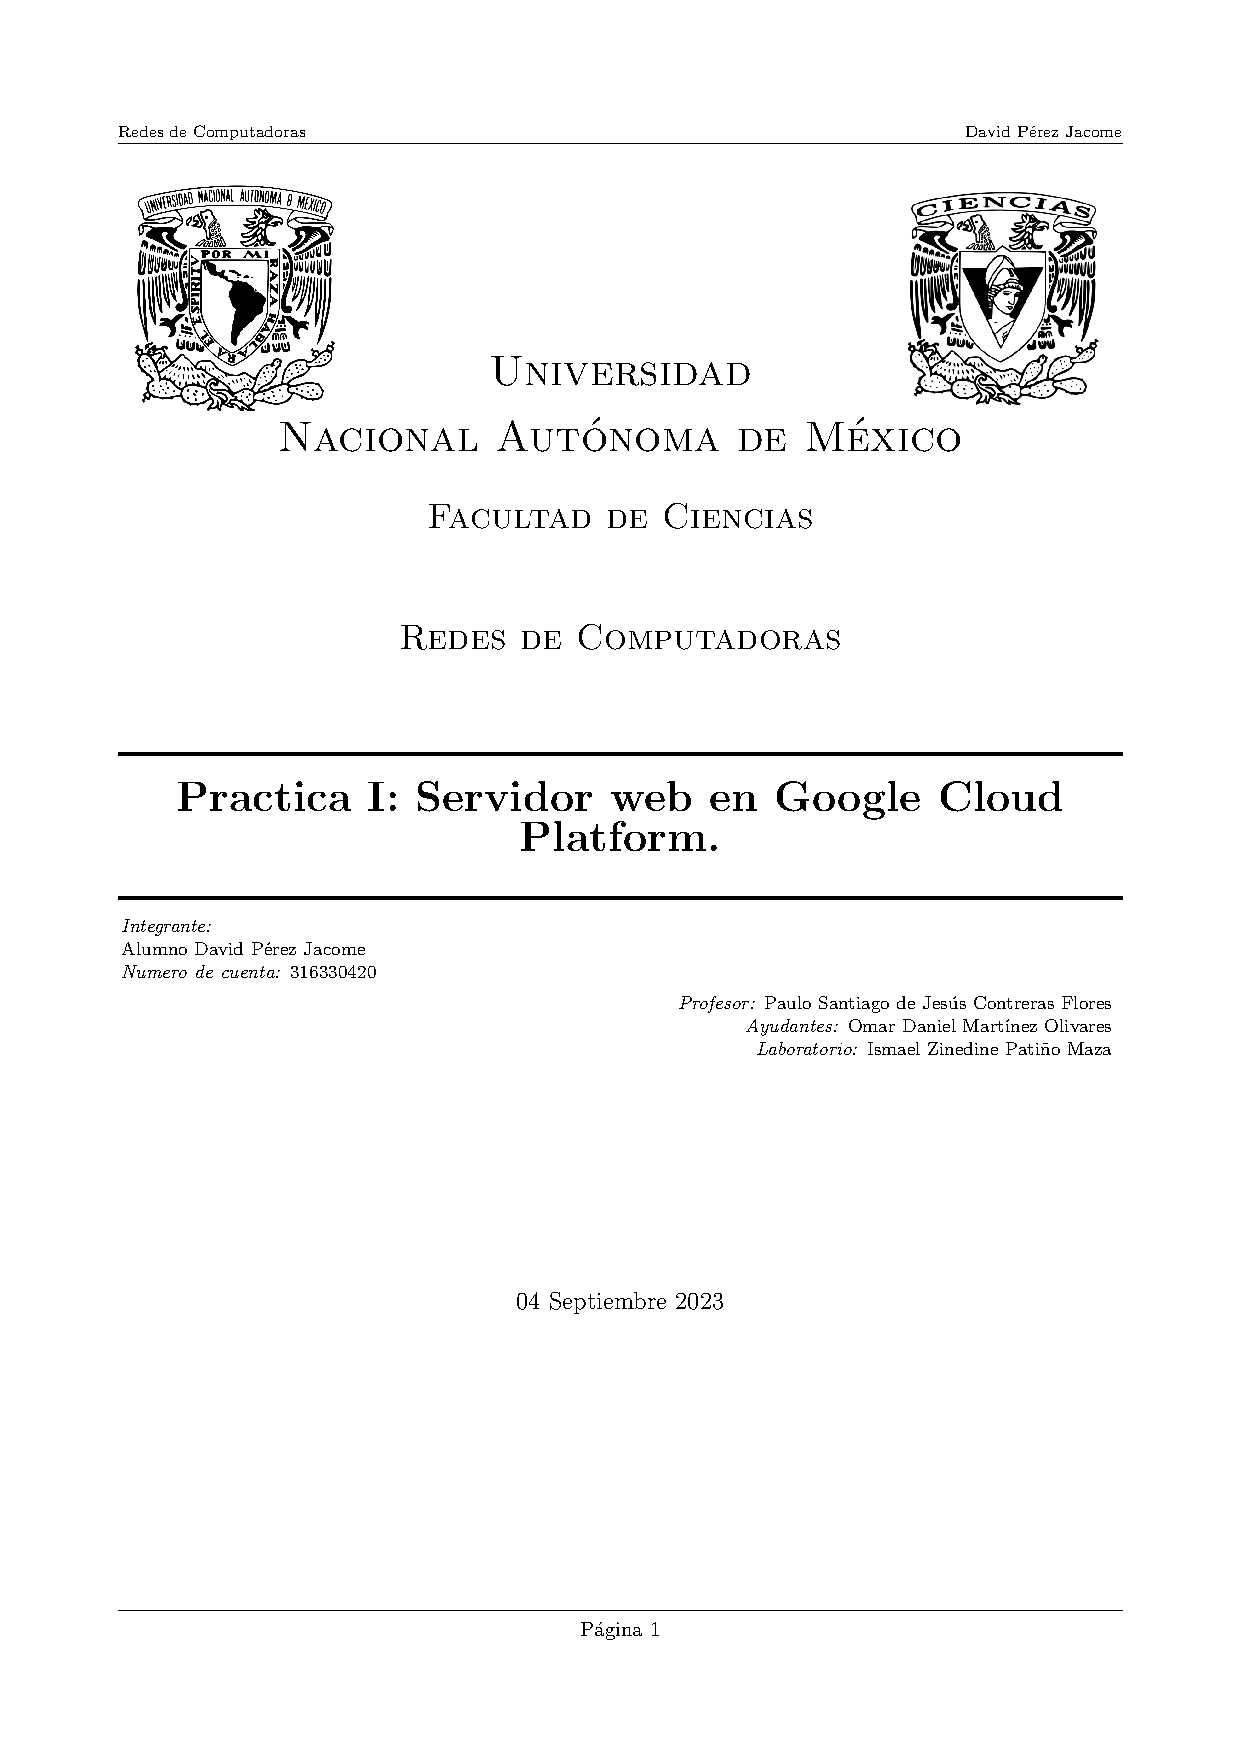
\includepdf{Portada.pdf}
{\color{red} \section*{\textbf{Practica I: Servidor web en Google Cloud Platform.}}}
\vspace{1em}

{\color{blue} \subsection*{\textbf{Objetivo.}}}
\vspace{1em}
El alumno instalará el servidor web Apache HTTPD, y publicará un formulario HTML en este servidor. Además, se familiarizará con el uso de los servicios GCP, VM Instances, Firewall Rules y Static public IP, proporcionados por Google Cloud.
\vspace{2em}

{\color{blue} \subsection*{\textbf{Introducción.}}}
\vspace{1em}
El protocolo HTTPS (HyperText Transfer Protocol Secure) es un protocolo de la Capa de aplicación que permite el envió de información cifrada usando los protocolos HTTP y SSL/TLS. El protocolo HTTP envía información en claro a través del medio, el protocolo SSL/TLS es el encargado de encapsular el protocolo HTTP para ser enviado de manera cifrada.
\vspace{2em}


{\color{blue} \subsection*{\textbf{Desarrollo.}}}
\vspace{1em}
\begin{enumerate}
    \item Creación de cuenta en google cloud.
    \item Creación y configuración de instacia.
    \item Conexión por SSH via web.
    \item Instalación del servidor Apache.
    \item Creación y asignación de reglas de firewall.
    \item Asiganación de IP publica fija.
    \item Visualización web.
    \item Asignación de un formulario web.
\end{enumerate}\\

Para iniciar con la practica lo primero que hicimos fue la creación de la instancia.\\
\textbf{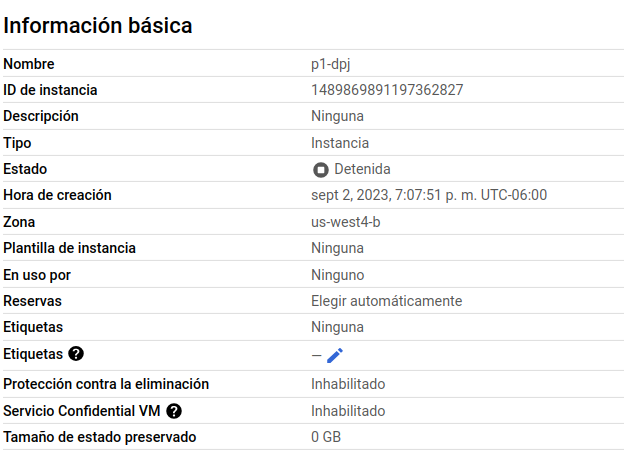
\includegraphics[scale = 0.40]{images/instancia de p1.png}}\\
Aqui podemos ver todos los datos importantes de la instancia para la practica 1, la cual por el momento esta detenida pero la nombramos \textbf{P1-dpj}, con zona \textbf{us-west4-b}. 
\vspace{2em}

Ahora procedemos a la instalación de apache2, esto lo realizamos desde la terminal de nuestra maquina virtual la cual al generar la instancia la definimos con las siguientes caracteristicas:\\
\textbf{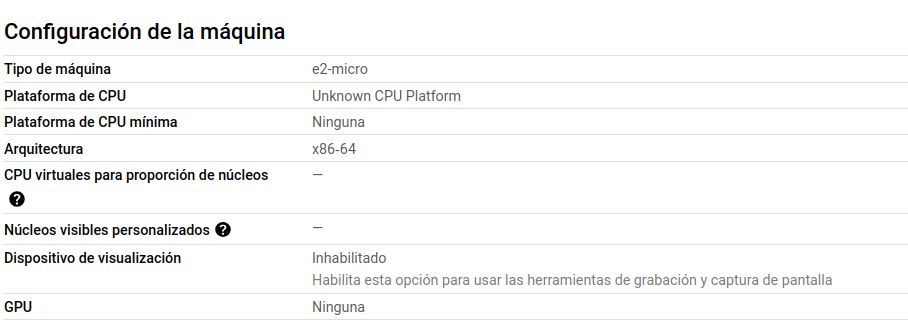
\includegraphics[scale = 0.40]{images/maquina virtual.png}}\\
Aqui podemos ver las caracteristica de la maquina virtual que nos ayudará a movernos y poder definir las conexiones de la instancia.\\

\textbf{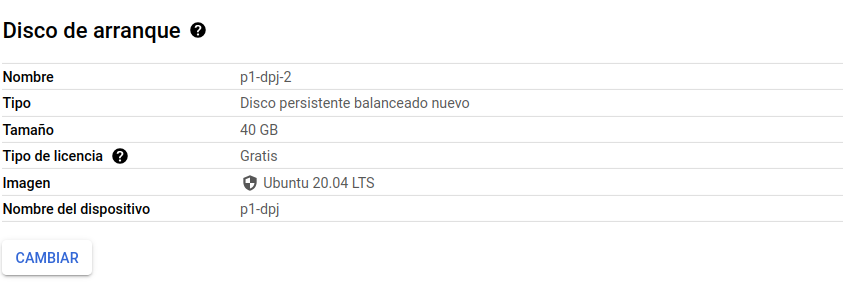
\includegraphics[scale = 0.40]{images/disco.png}}\\
Aqui más especificaciones.\\

Ahora isntalamos apache2\\

\textbf{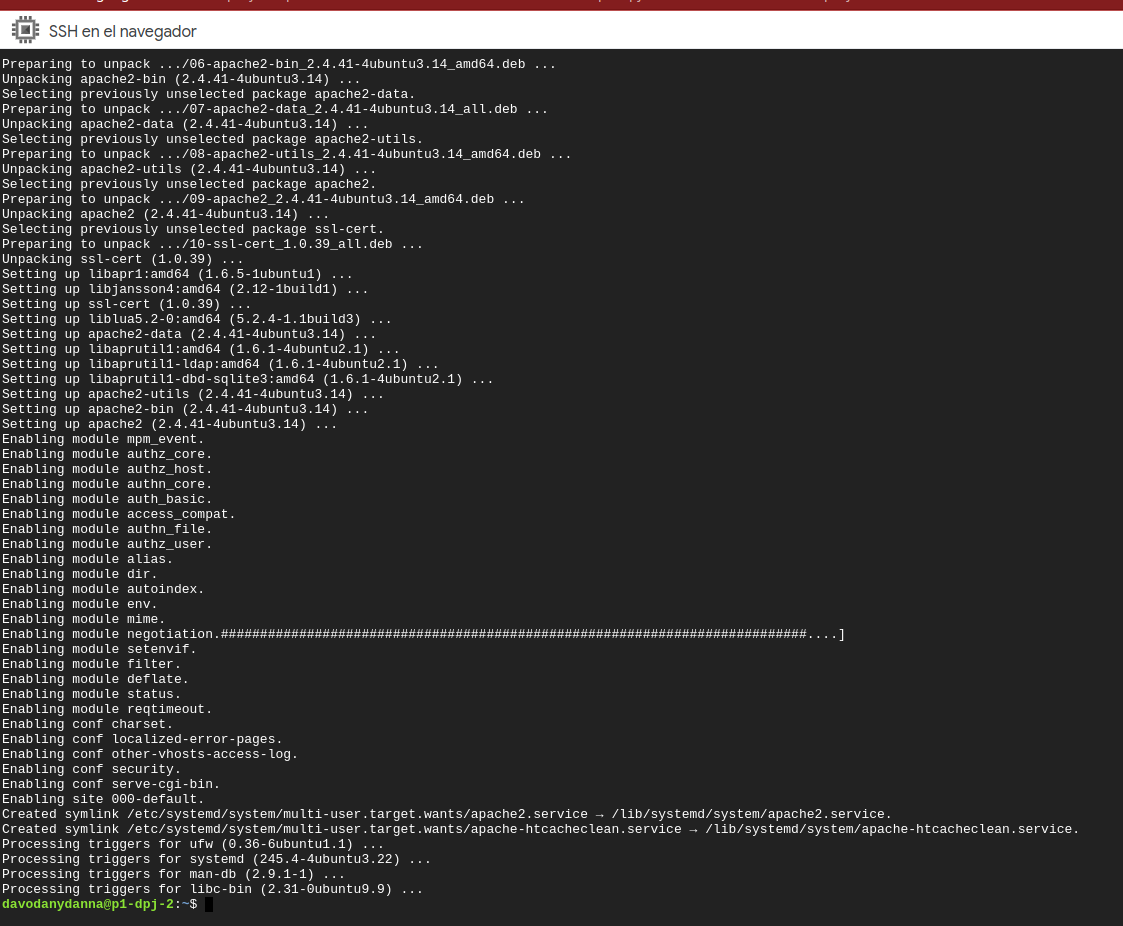
\includegraphics[scale = 0.40]{images/apache.png}}\\

y tambien definimos las reglas de firewall para despues no editarlas aparte\\

\textbf{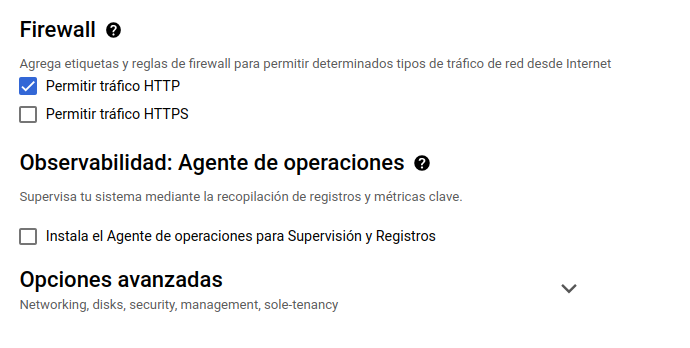
\includegraphics[scale = 0.40]{images/firewall.png}}\\

Ahora vemos nuestra instancia creada y corriendo:\\

\textbf{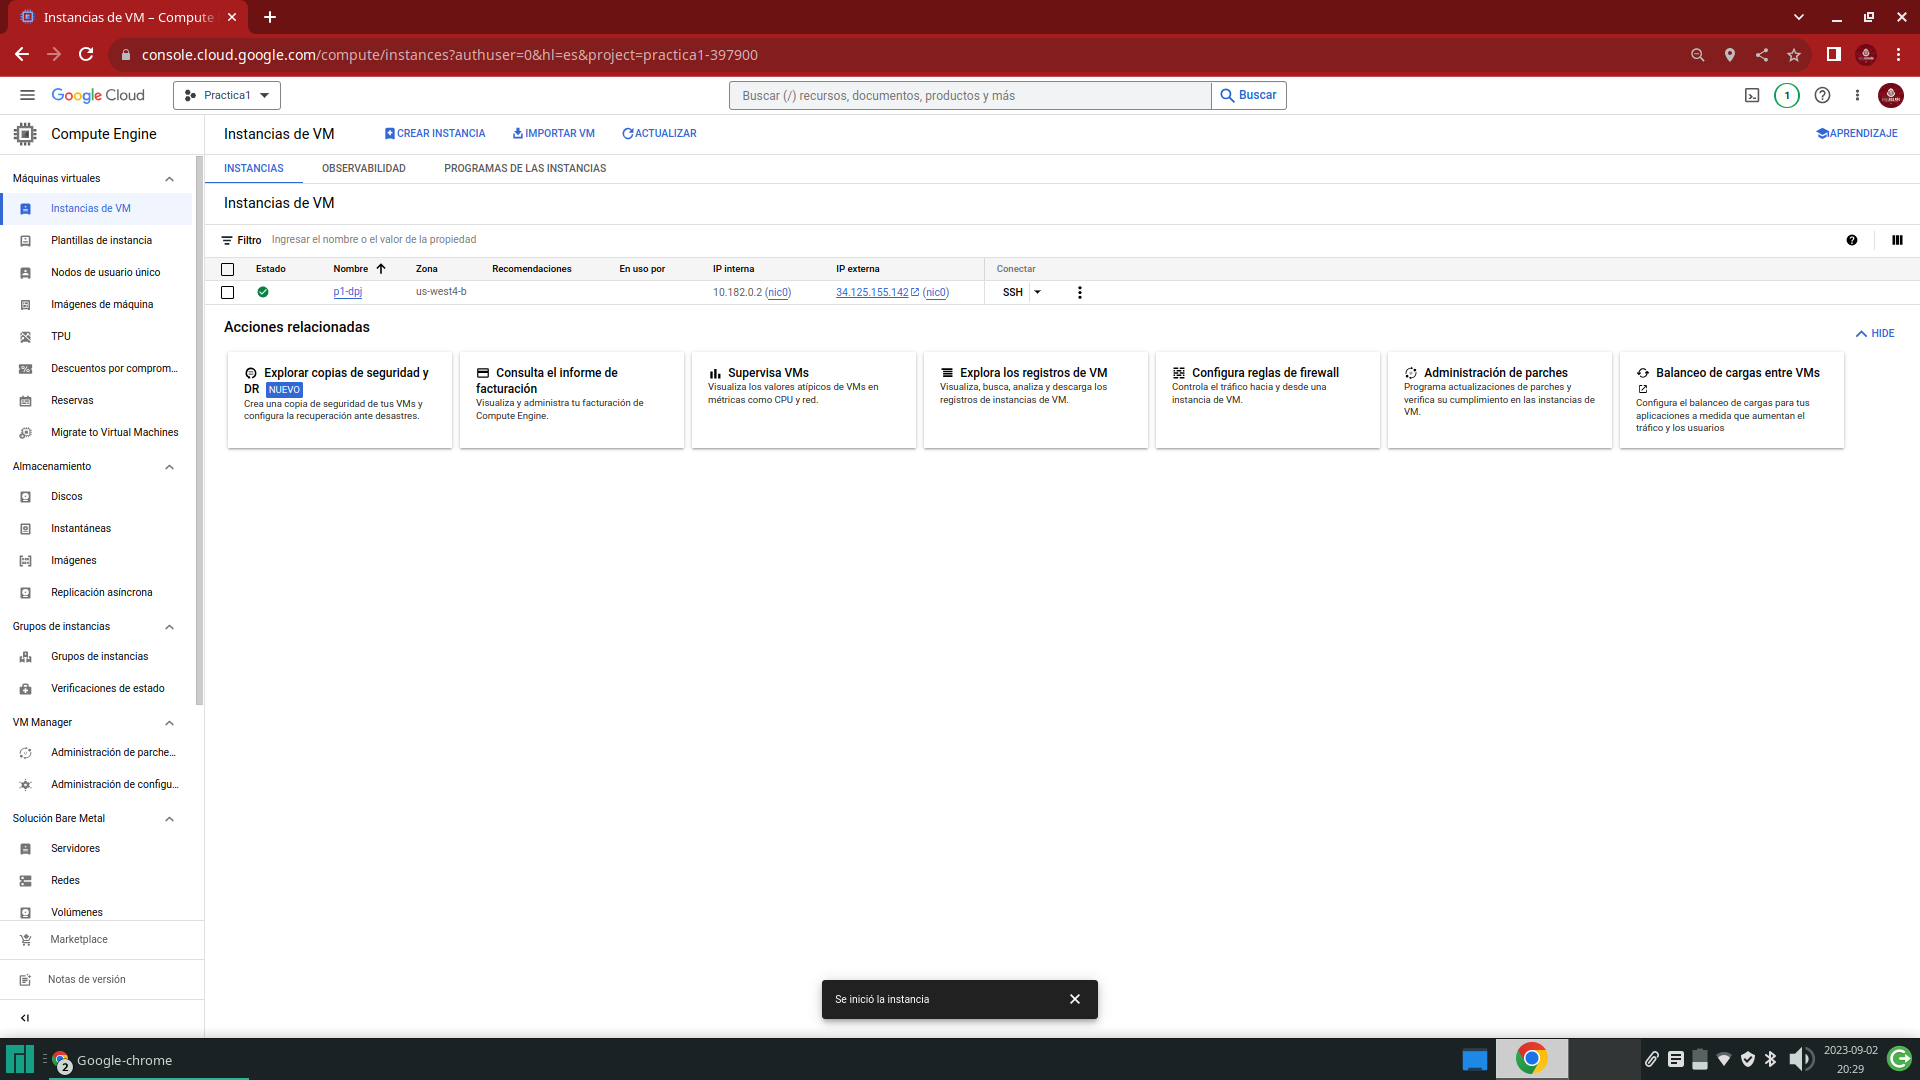
\includegraphics[scale = 0.40]{images/instancia creada y corriendo.png}}\\


Despues para terminar creamos nuestro formulario de inicio de sesión en HTML, el cual quedo de la siguiente manera:\\
\textbf{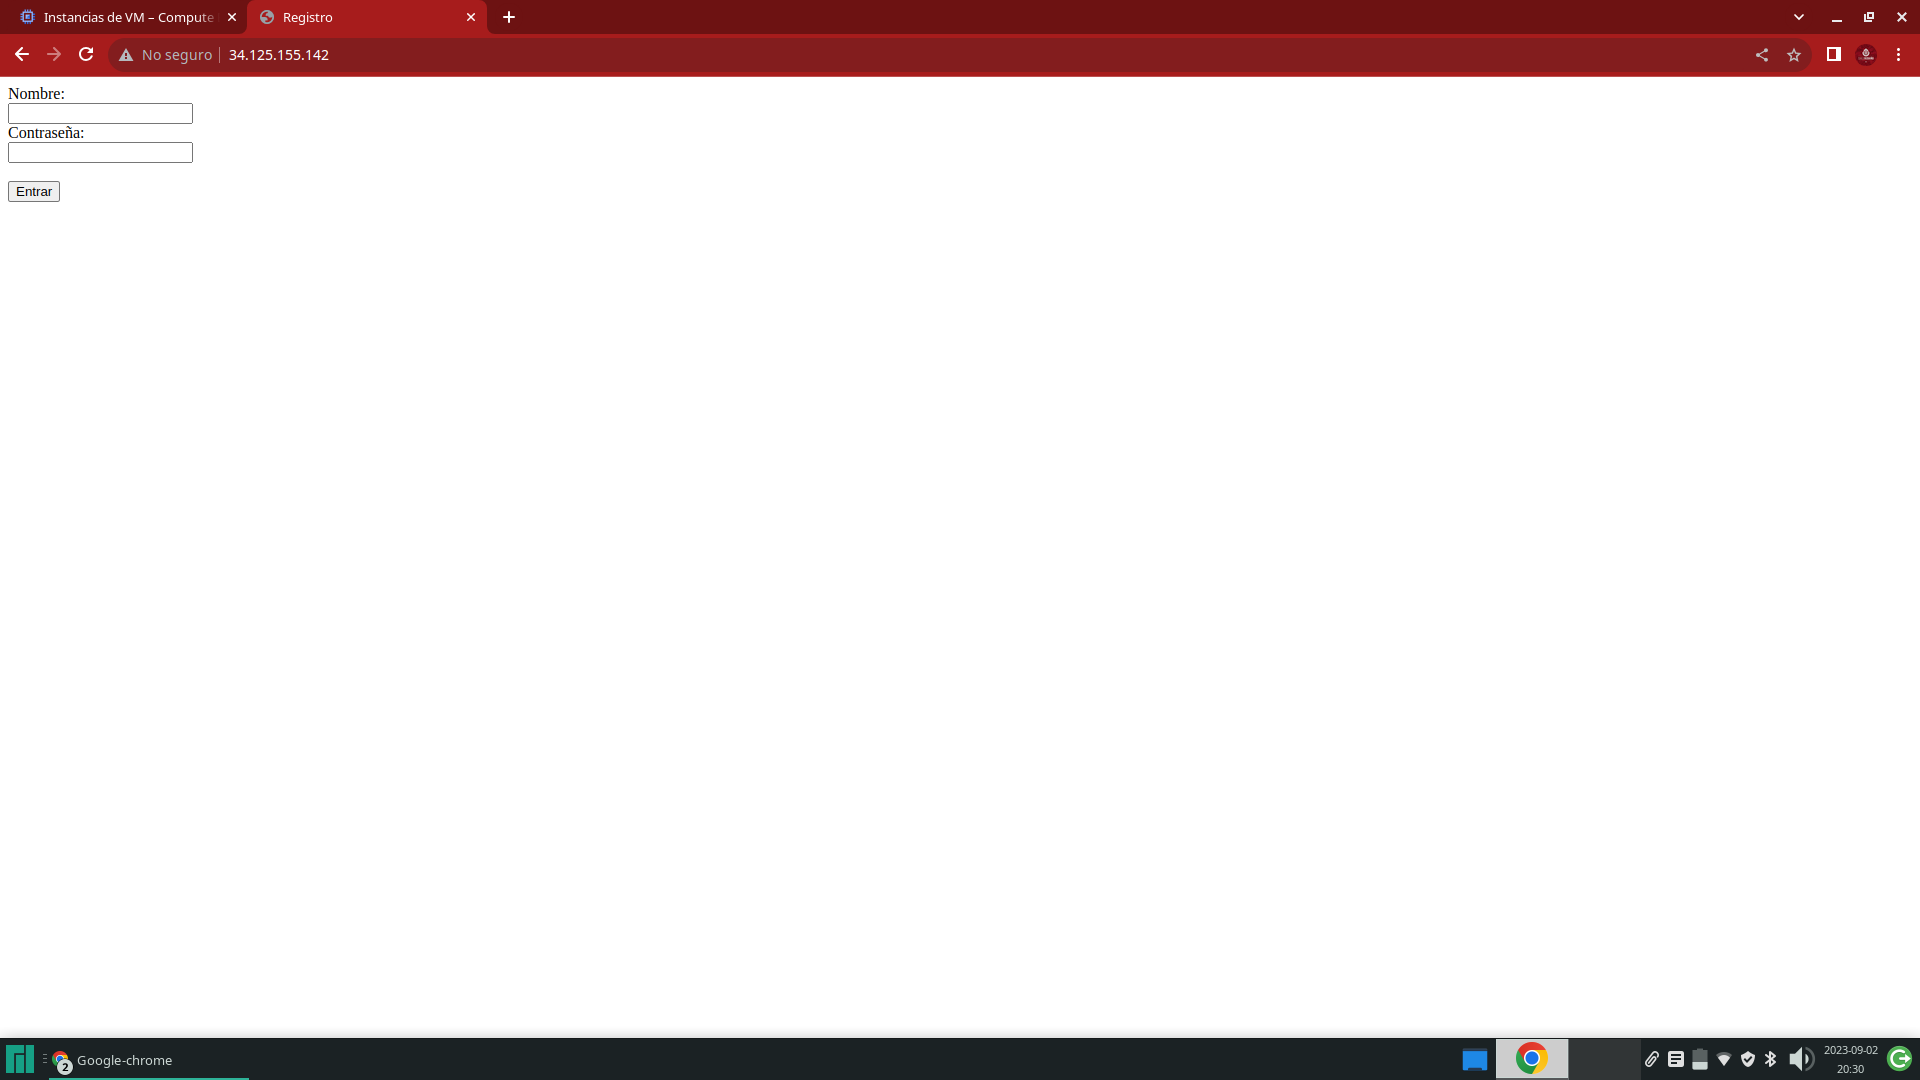
\includegraphics[scale = 0.25]{images/Formulario.png}}\\

{\color{blue} \subsection*{\textbf{Evaluación.}}}
\vspace{1em}
\begin{enumerate}
    \item ¿Qué es el concepto de nube y a qué se refiere el término IaaS?\\
    \textbf{La nube hace referencia a los servidores a los que se accede a través de Internet, y al software y bases de datos que se ejecutan en esos servidores.
    La IaaS es parte de la nube y consiste en alquilar servicios de infraestructura en la nube como servicios individuales de un proveedor de servicios en la nube, incluidos servidores, máquinas virtuales, recursos de redes y almacenamiento, como un prestamo de los servidores a grandes empresas. }
    \item ¿Qué ventajas observas al utilizar la infraestructura que utilizamos en esta práctica?\\
    \textbf{Pues a mi parecer es muy facil de usar y es muy conveniente, además se ajusta a nuestras necesidades como estudiantes, no es mi más ni menos, es lo ideal, la verdad me gustó mucho.}
    \item Colocar comentarios sobre la práctica\\
    \textbf{A decir verdad, nunca habia usado servicios como estos ni conocia mucho respecto a ello y a mi parecer lo senti más facil de usar que el servicio anterior de oracle, además me guato mucho el crear instancias de 0 y ver como es que funcionan los servidores.}
\end{enumerate}

\end{document}